\documentclass[resume]{subfiles}


\begin{document}
\section{ADC / DAC}

\section{ADC 3}

\subsection{Discrétisation}
Valeur du signal continu pris à des temps précis (sample)
Après l'échantillonnage, la valeur est quantifiée sur une valeur de $2^n$
\subsubsection{Idéal}
\begin{equation}
x_s(t) = \sum^{+\infty}_{k=-\infty} x(kT_s)\cdot \delta(t-kT_s) = x(t)\cdot \sum^{+\infty}_{k=-\infty} \delta(t-kT_s)
\end{equation}
\subsubsection{Critère de Nyquist}
$f_s > 2(f_a-f_b)$ avec $f_a$ limite haute de la BW du signal et $f_b$ limite basse de la BW

\subsection{Aliasing}
L'échantillonnage d'un signal provoque une répétition du spectre du signal autour de $f_s$ et de multiples de $f_s$.

\subsection{Signal Noise Ratio}
\begin{itemize}
\item Bruit de quantification RMS $N_{RMS} = \frac{V_{LSB}}{\sqrt{12}}$
\item Tension sinus FullScale $S_{RMS}\frac{V_{LSB}}{\sqrt{2}}\cdot \frac{2^N}{2}$
\item $SNR = 20log(\frac{S_{RMS}}{N_{RMS}}) = 20log(\sqrt{\frac{12}{8}}) + 20log(2^N)$
\item En dB $SNR = 6.02N + 1.76 $
\end{itemize}

\subsection{Process gain}
C'est lorsque l'on utilise pas toute la bande de 0 à $f_s/2$
le gain pour un sinus FullScale est le suivant.
\begin{equation}
SNR = 6.02N + 1.76 + 10log(\frac{f_s}{2\cdot BW})
\end{equation}

\subsection{Sur-échantillonnage}
\begin{equation}
SNR = 6.02N + 1.76 + 10log(OSR)
\end{equation}
Meilleur de 3dB à chaque fois que la $f_s$ double.

\subsection{Conversion Sigma-Delta}
\paragraph{Modulateur de premier ordre}
\subparagraph{Analogique}
\begin{figure}[H]
    \centering
    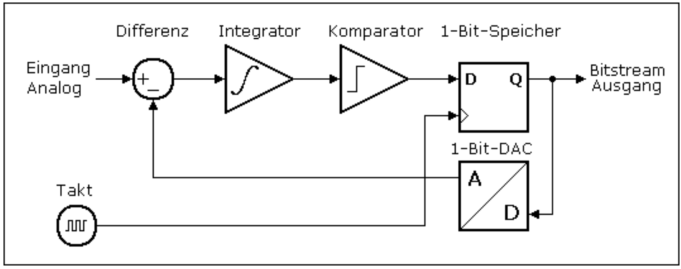
\includegraphics[width=0.8\columnwidth]{../images/OpAmp1/1ordreSD.png}
\end{figure}

\subparagraph{Digital}
\begin{figure}[H]
    \centering
    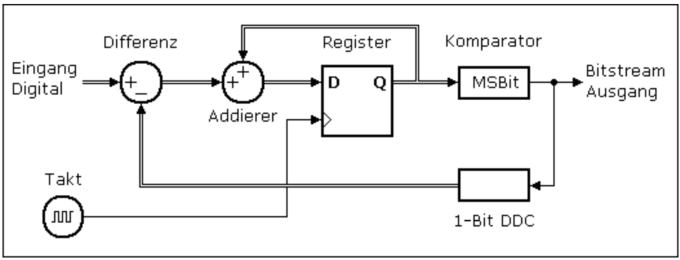
\includegraphics[width=0.8\columnwidth]{../images/OpAmp1/1ordreSDnum.png}
\end{figure}

\paragraph{Modulateur du deuxième ordre}
\begin{figure}[H]
    \centering
    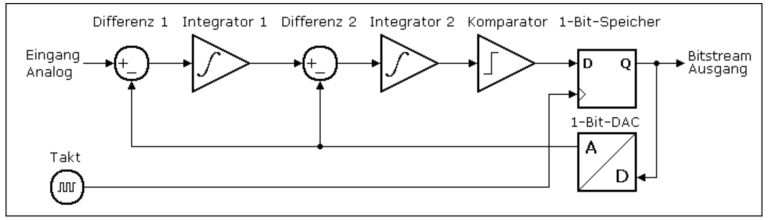
\includegraphics[width=0.8\columnwidth]{../images/OpAmp1/2ordreSD.png}
\end{figure}

\subsubsection{Sur-échantillonnage pour SD}
\begin{figure}[H]
    \centering
    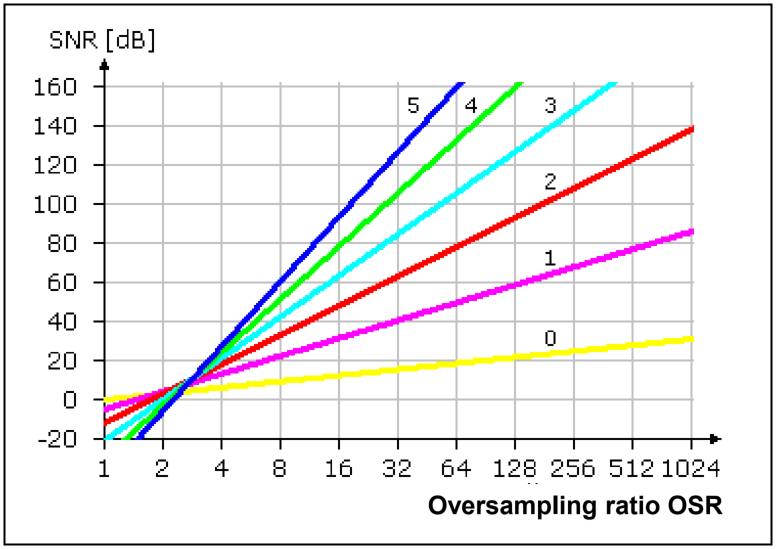
\includegraphics[width=0.8\columnwidth]{../images/OpAmp1/oversampling.png}
\end{figure}







\end{document}